\chapter{无约束非光滑目标的求解}
\label{chap:nonsmooth-optimization}

本章始终评价同一个原问题$\min_{\bm w\in\mathbb R^d}F(\bm w)$。绝对值损失和$\ell_1$稀疏正则项在尖点处没有经典导数，普通梯度更新在那里失去定义；减小步长并不能补出不存在的导数，问题在于重新确定可计算的更新信息。

面对同一个非光滑目标，有四条彼此不同的求解路线。次梯度法每轮只选取一条全域支撑斜率，显式更新，代价小但不保证本轮下降；邻近方法把难处理的非光滑项完整保留，加二次距离后求一个子问题；光滑化用可控的逼近偏差把尖点替换成光滑曲线，再调用第11章的方法；束方法积累多条支撑切面构造下模型，用原目标决定是否移动稳定中心。它们不是互斥的函数集合：同一目标可以同时有易求的邻近项和有限最大值结构。本章先在12.1建立共用的凸支撑，12.2—12.5分别给出四类方法的一轮实现与专属分析，12.6回到原目标的存在、唯一与最优性，12.7比较收敛速度与精度，12.8讨论迭代过程与数值敏感度。本章先分析精确次梯度与明确精度的子问题；读数误差与第14章的抽样留到那里处理。

\section{凸次梯度与支撑信息}

先看$f(x)=|x|$：零点左侧斜率为$-1$、右侧为$1$，一个经典导数无法同时匹配两侧变化。与光滑凸函数可微点处切线下界对照，自然的做法是在尖点保留全部“全域有效”的支撑斜率。

\begin{definition}[凸次梯度与次微分]
\label{def:opt-convex-subgradient}
设$f:\mathbb R^d\to\mathbb R\cup\{+\infty\}$为适当凸函数，$\bm u$为有限值点。向量$\bm g$若满足
\[
 f(\bm v)\geq f(\bm u)+\langle\bm g,\bm v-\bm u\rangle
 \quad\text{对所有 }\bm v
\]
就称为$f$在$\bm u$处的\term{次梯度}（subgradient）；全部这样的向量组成\term{次微分}（subdifferential）$\partial f(\bm u)$。
\end{definition}

次梯度是一组全域有效的仿射下界斜率，集合可以为空，定义不保证任意边界点都能选出更新向量。对$|x|$：正半轴次微分为$\{1\}$，负半轴为$\{-1\}$，零点则由$|v|\geq gv$对正、负$v$的限制得到$\partial|x|(0)=[-1,1]$。这个完整区间是后面零向量最优性判据的依据，不能把其中任意一个数当作“零点导数”。

即使讨论两个适当凸函数之和，也不能无条件写$\partial(f+r)=\partial f+\partial r$：求和等式需要定义域接触等额外条件（Moreau--Rockafellar条件）。本章需要的邻近最优性关系都直接从函数比较证明，只依赖单函数的全域支撑。

\section{次梯度法}
\label{sec:opt-subgradient-methods}

当凸目标在尖点没有梯度、却能给出函数值和一条全域支撑斜率时，次梯度法沿负支撑向量显式更新，避免每轮求解完整子问题。

\subsection{支撑更新与实际返回点}

给定初值和正步长，逐轮选取$\bm g^{(t)}\in\partial f(\bm w^{(t)})$，更新
\begin{equation}
 \bm w^{(t+1)}=\bm w^{(t)}-\eta^{(t)}\bm g^{(t)}.
 \label{eq:opt-subgradient-update}
\end{equation}
扩展实值目标还须核验更新留在有效定义域，不能用无投影公式代替域检查。支撑斜率不保证给原目标的下降方向，所以实现必须同时规定返回对象：保存历史最佳目标点，或维护步长加权平均
\[
 \bar{\bm w}^{(T)}
 =\frac{\sum_{t<T}\eta^{(t)}\bm w^{(t)}}{\sum_{t<T}\eta^{(t)}}.
\]
执行次序是先用当前函数值更新最佳点、累计当前点的加权和，再计算下一点；距离保证针对被查询的旧点。

\subsection{预算停止与最优性核验}

停止时报告实际返回对象及其目标值：有可信最优值下界时核验目标差，否则只报告预算与已满足的界条件。某轮不降不能自动判为失败；选到零次梯度可核验当前点全局最优，但任选的非零次梯度范数不是唯一的驻点残差，步长变小或点变化小也不证明参数全序列收敛。

\subsection{支撑方向与单步变化的边界}

先用$|x|$从$0.2$以步长$1$走到$-0.8$说明大步会跨过尖点使目标上升。再把“跨过最小点”与“方向本身不下降”分开：在$f(x,y)=|x|+y/2$的原点取$\bm g=(1,1/2)^\top$，沿$-t\bm g$的真实值为$3t/4$，而支撑下界为$-5t/4$——任意小的正步都使真实目标上升，全域下界却仍然有效。

图~\ref{fig:vol1-add-subgradient-not-descent}沿负次梯度方向直接比较真实函数值与支撑下界。
\begin{figure}[!htb]
  \centering
  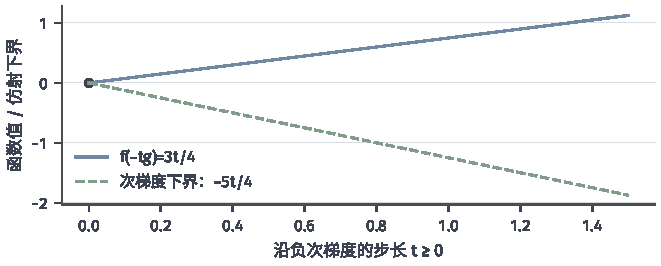
\includegraphics[width=112mm]{figures/00-shared/mathematical-preliminaries-upper/00-shared/matplotlib/mathematical-language-combinatorics-analysis-optimization-comprehension-additions/subgradient-not-descent.pdf}
  \caption{令$f(x,y)=|x|+y/2$、$\bm g=(1,1/2)^\top$。沿$-t\bm g$、$t\geq0$移动时，真实函数值为$3t/4$，该次梯度给出的仿射下界为$-5t/4$。下界始终有效，所选方向却对任意$t>0$上升。}
  \label{fig:vol1-add-subgradient-not-descent}
\end{figure}

再用$f(x,y)=|x|+|y|$检验集合值选择：在$(0.5,0)$处次微分为$\{1\}\times[-1,1]$，选$(1,0)^\top$一步跨到对称点使目标不变；在原点选$(1,1)^\top$则使目标上升。这些反例限定的是逐轮下降保证，总体进展改由历史最佳点或加权平均评价。

\subsection{返回点目标差与预算步长}

设$f$凸、最小点$\bm w^\star$存在、$\|\bm w^{(0)}-\bm w^\star\|_2\leq R$，且实际选出的每个次梯度范数不超过$G$。展开距离平方并用全域支撑，得
\[
 2\eta^{(t)}[f(\bm w^{(t)})-f^\star]
 \leq\|\bm w^{(t)}-\bm w^\star\|_2^2
 -\|\bm w^{(t+1)}-\bm w^\star\|_2^2
 +(\eta^{(t)})^2G^2.
\]
求和后，历史最佳点与步长加权平均点共用目标差界
\begin{equation}
 \min_{t<T}f(\bm w^{(t)})-f^\star
 \leq
 \frac{R^2+G^2\sum_{t<T}(\eta^{(t)})^2}
 {2\sum_{t<T}\eta^{(t)}}.
 \label{eq:opt-subgradient-finite-rate}
\end{equation}
预算$T$已知、$R,G>0$时取$\eta=R/(G\sqrt T)$，两项平衡给$RG/\sqrt T$；这是特定返回点的速率，不是每轮单调下降。预算未知时取$\eta^{(t)}=R/(G\sqrt{t+1})$，累计步长按$\sqrt T$增长、平方步长和按$\log T$增长，给$O(\log T/\sqrt T)$。真正要求的是分母相对初始距离项与平方步长项持续增大；有效定义域、次梯度可选性及有界$G$都须单独核验。实际路径长度为$\sum\eta^{(t)}\|\bm g^{(t)}\|_2$，还含次梯度范数，不能用累计步长代替。

\section{邻近梯度法与邻近点法}

\subsection{邻近算子与可计算的非光滑项}

与其在多个支撑斜率中只挑一条，不如完整保留非光滑项，再加入离中心的平方距离代价，让尖点两侧的形状一起决定走到哪。

\begin{definition}[邻近算子]
\label{def:opt-proximal-operator}
设$r:\mathbb R^d\to\mathbb R\cup\{+\infty\}$适当、下半连续且凸，$\eta>0$。其\term{邻近算子}（proximal operator，近端算子）为
\[
 \operatorname{prox}_{\eta r}(\bm z)
 =\arg\min_{\bm w}\left\{
 r(\bm w)+\frac{1}{2\eta}\lVert\bm w-\bm z\rVert_2^2
 \right\}.
\]
\end{definition}

这里的$\eta$先只是子问题中的权重参数，算法使用它时才成为步长；“闭凸函数”的闭指下半连续，不要求有效定义域本身闭。只最小化$r$可能远离当前点，只最小化距离则不改善$r$，两项平衡给出邻近子问题。

\paragraph{存在唯一与非扩张。}
在适当、下半连续、凸与$\eta>0$条件下，二次距离项是$1/\eta$强凸的。取有限值候选，先可证$r$的负向增长至多线性（在紧球上有下界即可），于是二次项支配远距离，子问题强制且强凸，每个中心有唯一输出。令$\bm p=\operatorname{prox}_{\eta r}(\bm z)$，最优性等价于
\begin{equation}
 \frac{\bm z-\bm p}{\eta}\in\partial r(\bm p),
 \label{eq:opt-prox-optimality}
\end{equation}
故斜率读取于新点。把两个中心$\bm x,\bm y$的最优性不等式相加，得
\begin{equation}
 \lVert\operatorname{prox}_{\eta r}(\bm x)
 -\operatorname{prox}_{\eta r}(\bm y)\rVert_2
 \leq\lVert\bm x-\bm y\rVert_2.
 \label{eq:opt-prox-nonexpansive}
\end{equation}
存在唯一、充要关系和非扩张性不等于子问题能够低成本求解。

\paragraph{软阈值。}
对$r(\bm w)=\lambda\|\bm w\|_1$、$\lambda\geq0$，逐坐标最小化得到\term{软阈值}
\begin{equation}
 [\operatorname{prox}_{\eta r}(\bm z)]_j
 =\operatorname{sign}(z_j)\max\{|z_j|-\eta\lambda,0\}.
 \label{eq:opt-soft-threshold}
\end{equation}
零区间来自子问题最优性所需斜率$z_j/\eta$落在$\lambda[-1,1]$，而不是任取一条次梯度走一步。例如$\bm z=(3,0.4,-2)^\top$与$\eta\lambda=1$输出$(2,0,-1)^\top$；同样输入下二次收缩$z/(1+\eta\lambda)$为$(1.5,0.2,-1)$，二者行为不同。

图~\ref{fig:vol1-add-proximal-balance}画出软阈值所解的完整子问题。
\begin{figure}[!htb]
  \centering
  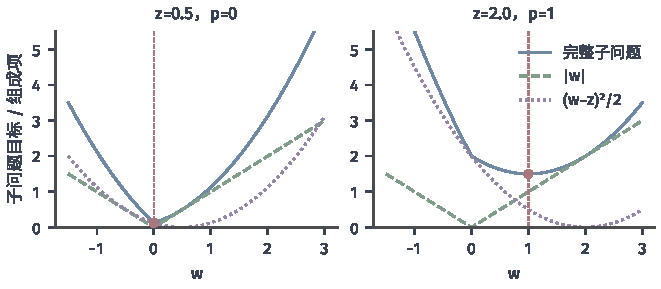
\includegraphics[width=112mm]{figures/00-shared/mathematical-preliminaries-upper/00-shared/matplotlib/mathematical-language-combinatorics-analysis-optimization-comprehension-additions/proximal-balance.pdf}
  \caption{固定$r(w)=|w|$与$\eta=1$，对$z=0.5,2$同时画完整子问题$|w|+(w-z)^2/2$及两项组成。蓝线是完整目标，绿虚线是尖点的$|w|$，紫点线是二次距离。最小点在$0$与$1$，精确最小点的斜率平衡见式~\eqref{eq:opt-prox-optimality}。}
  \label{fig:vol1-add-proximal-balance}
\end{figure}

\subsection{邻近梯度法}

对复合目标$F=f+r$，只对易求梯度的$f$作一阶加二次近似，完整保留$r$，配方后得到
\begin{equation}
 \bm w^{(t+1)}
 =\operatorname{prox}_{\eta r}\!\left(
 \bm w^{(t)}-\eta\nabla f(\bm w^{(t)})\right).
 \label{eq:opt-proximal-gradient-update}
\end{equation}
一轮依次为：在当前有效点求$f$的梯度，形成中心，求$r$的邻近解，核验后接受；回溯试探要重算邻近解。对共同二次目标加$\lambda\|\bm w\|_1$，从$(2,2)$以$\eta=1/16$先到$(15/8,0)$再软阈值，得$(\max\{15/8-\lambda/16,0\},0)$。

\paragraph{原目标下降。}
令$\bm d=\bm w^+-\bm w$，由式~\eqref{eq:opt-prox-optimality}有$-\nabla f(\bm w)-\bm d/\eta\in\partial r(\bm w^+)$。把该支撑不等式用于旧点，再与$f$的光滑上界相加：
\begin{equation}
 F(\bm w^+)\leq F(\bm w)
 -\left(\frac1\eta-\frac L2\right)\|\bm d\|_2^2.
 \label{eq:opt-proximal-gradient-descent}
\end{equation}
此式不要求$f$凸，$0<\eta\leq1/L$即保证下降。未知$L$时增大二次模型系数回溯，域外候选直接拒绝，每次试探都重求邻近解。

\paragraph{梯度映射作为停止量。}
定义可计算的邻近梯度映射
\[
 \bm G_\eta(\bm w)=\frac{\bm w-\bm w^+}{\eta}.
\]
$\bm G_\eta(\bm w)=\bm0$当且仅当$0\in\nabla f(\bm w)+\partial r(\bm w)$，即复合临界条件。属于新点次微分的向量$\bm G_\eta(\bm w)+\nabla f(\bm w^+)-\nabla f(\bm w)$的范数不超过$(1+L\eta)\|\bm G_\eta(\bm w)\|_2$，故旧点映射残差控制新点驻点性。下有界、固定$\eta\leq1/L$时累加式~\eqref{eq:opt-proximal-gradient-descent}给历史最小平方残差$O(1/T)$（范数$O(1/\sqrt T)$）；非凸时这是驻点残差而非全局目标差。

\paragraph{凸复合目标的最后一点目标差。}
再要求$f$凸、最小点存在。旧点凸下界、新点光滑上界与$r$的新点支撑组合成三点不等式
\[
 F(\bm w^+)-F(\bm v)
 \leq\frac{1}{2\eta}\bigl(
 \|\bm w-\bm v\|_2^2-\|\bm w^+-\bm v\|_2^2
 \bigr),
\]
取$\bm v=\bm w^\star$求和，得
\[
 F(\bm w^{(T)})-F^\star
 \leq\frac{\|\bm w^{(0)}-\bm w^\star\|_2^2}{2\eta T}.
\]

\paragraph{固定度量变体。}
若使用11.1.2的固定预条件$\bm P\succ\bm0$，距离项必须匹配：令$\bm z=\bm w-\eta\bm P\nabla f(\bm w)$，子问题为
\[
 \bm w^+=\arg\min_{\bm u}\left\{
 r(\bm u)+\frac{1}{2\eta}\|\bm u-\bm z\|_{\bm P^{-1}}^2
 \right\},\quad
 \|\bm u\|_{\bm P^{-1}}^2=\bm u^\top\bm P^{-1}\bm u.
\]
取$\bm u=\bm P^{1/2}\bm v$即化为欧氏邻近问题；对角$\bm P$与$r=\lambda\|\cdot\|_1$给逐坐标阈值$\eta p_j\lambda$，一般耦合$\bm P$则失去便宜的逐坐标软阈值。只换中心而不换距离，不能沿用欧氏残差界。

\subsection{邻近点法}

若整个目标的邻近问题可解，\term{邻近点法}（proximal point method，近端点法）直接做隐式更新：
\[
 \bm w^{(t+1)}
 =\operatorname{prox}_{\eta^{(t)}F}(\bm w^{(t)}).
\]
每轮固定旧点，组装$F$加距离项，求完整最小点，最优性$(\bm w^{(t)}-\bm w^{(t+1)})/\eta^{(t)}\in\partial F(\bm w^{(t+1)})$中的斜率位于新点。以旧点为可行候选立即得到
\[
 F(\bm w^{(t+1)})
 +\frac{1}{2\eta^{(t)}}\|\bm w^{(t+1)}-\bm w^{(t)}\|_2^2
 \leq F(\bm w^{(t)}).
\]
这里没有由$L$决定的步长上限，但每步可能要求解一个与原问题几乎同样困难的子问题；邻近梯度只线性化$f$正是为减少这一负担。$F$适当闭凸、最小点存在、固定$\eta>0$且子问题精确求解时，最后一点目标差同样为$\|\bm w^{(0)}-\bm w^\star\|_2^2/(2\eta T)$。

\paragraph{弱凸情形的工具边界。}
若原函数$f$为全空间\term{$\rho$弱凸}，即$f+\rho\|\cdot\|_2^2/2$凸，则$\rho>0$时取$0<\eta<1/\rho$，邻近子问题的强凸常数为$1/\eta-\rho$，仍有唯一输出；$\rho=0$时任意正步长适用。但凸邻近的非扩张性不再成立：$f(x)=-\rho x^2/2$的邻近解为$z/(1-\eta\rho)$，反而放大中心扰动。这里建立的只是方法工具的可解性，原$f$有无全局最小点仍由12.6回答。

\section{光滑化逼近法}

当非光滑项具有有限仿射最大值结构、又没有便宜邻近算子时，可以用可控偏差把它替换成光滑函数。固定
\[
 F(\bm w)=\phi(\bm w)+\max_{1\leq i\leq m}\{\bm a_i^\top\bm w+b_i\},
\]
其中$\phi$全空间凸且$L_\phi$光滑。定义$\nu>0$的熵光滑化
\[
 F_\nu(\bm w)=\phi(\bm w)
 +\nu\log\sum_{i=1}^m
 \exp\frac{\bm a_i^\top\bm w+b_i}{\nu}.
\]
把最大仿射值提出指数外，得到全空间一致界
\begin{equation}
 F(\bm w)\leq F_\nu(\bm w)\leq F(\bm w)+\nu\log m.
 \label{eq:opt-smoothing-gap}
\end{equation}
令软权重
\[
 p_i(\bm w)=
 \frac{\exp[(\bm a_i^\top\bm w+b_i)/\nu]}
 {\sum_j\exp[(\bm a_j^\top\bm w+b_j)/\nu]},
\]
则$\nabla F_\nu=\nabla\phi+\sum_i p_i\bm a_i$：这些权重是同一点所有仿射片的软组合，不是原目标的任取次梯度。光滑化最大值的Hessian为权重协方差$\sum_i p_i(\bm a_i-\bar{\bm a})(\bm a_i-\bar{\bm a})^\top$，以$M_A=\max_i\|\bm a_i\|_2$控制得梯度Lipschitz上界$L_\phi+M_A^2/\nu$。减小$\nu$缩小偏差，却增大曲率、缩小可用步长。

给定原目标差要求$\varepsilon$，取$\nu=\varepsilon/(2\log m)$使偏差不超过$\varepsilon/2$，再把光滑求解误差预算设为$\delta\leq\varepsilon/2$。固定$\nu$后可用普通梯度（复杂度$O(\varepsilon^{-2})$）或凸加速程序（$O(\varepsilon^{-1})$）达到$\delta$；一致逼近保证
\[
 F(\widehat{\bm w})-F^\star
 \leq[F_\nu(\widehat{\bm w})-F_\nu^\star]+\nu\log m.
\]
固定$\nu$时增加迭代只减小优化误差、消不去$\nu\log m$；重新减小$\nu$必须重估$L_\nu$，不能沿用旧步长。对$F(x)=|x|$，光滑化为$\nu\log(e^{x/\nu}+e^{-x/\nu})$、梯度为$\tanh(x/\nu)$，跨尖点时实际沿光滑替代更新。这一速度承诺依赖显式最大值结构与全梯度，不适用于任意非光滑黑盒。

\section{束方法}

若凸目标能返回精确函数值与次梯度、却没有易解的邻近算子，单条支撑更新浪费了过去查询揭示的形状。束方法积累全部支撑切面构造下模型，加至稳定中心的距离项求候选，再查原函数决定是否移动中心。

固定$F:\mathbb R^d\to\mathbb R$有限凸，预言器在每个查询点返回精确$F$与$\bm g_j\in\partial F(\bm y_j)$。第$k$轮的束模型为
\[
 m_k(\bm w)=\max_{0\leq j\leq k}
 \{F(\bm y_j)+\bm g_j^\top(\bm w-\bm y_j)\}\leq F(\bm w),
\]
候选由
\[
 \bm y_{k+1}=\arg\min_{\bm w}\left\{
 m_k(\bm w)+\frac{1}{2\tau}\|\bm w-\bm x_k\|_2^2
 \right\}
\]
唯一给出（有限仿射片加正二次项强制且强凸），可用带辅助变量$q$的凸二次规划求解。定义未加二次项的预测下降$\Delta_k=F(\bm x_k)-m_k(\bm y_{k+1})\geq0$；查询$F(\bm y_{k+1})$后，若
\[
 F(\bm x_k)-F(\bm y_{k+1})\geq\beta\Delta_k
\]
则接受为实质步、移动稳定中心，否则为空步、中心不变；两种情况都把新切面加入束。空步消耗查询并改进模型，却不移动中心。

令$\bm s_k=(\bm x_k-\bm y_{k+1})/\tau$，模型最优性与中心处模型精确性推出带误差支撑
\[
 F(\bm w)\geq F(\bm x_k)+\bm s_k^\top(\bm w-\bm x_k)-e_k,
 \qquad e_k=\Delta_k-\tau\|\bm s_k\|_2^2\geq0.
\]
若已知某最小点满足$\|\bm x_k-\bm w^\star\|\leq R_k$，则$F(\bm x_k)-F^\star\leq e_k+R_k\|\bm s_k\|_2$，可作停止证书；$\Delta_k=0$给出精确全局最优，$\Delta_k$小本身不等于目标差。在全空间$M$-Lipschitz、固定参数和有界中心距离等条件下，全记忆邻近束方法让$\varepsilon\downarrow0$时实质步数为$O(\varepsilon^{-1})$、空步数为$O(\varepsilon^{-3})$；不能剔除空步后宣称总查询数为$O(\varepsilon^{-1})$，一次外层计数也不含模型二次规划的内迭代。

\section{原目标最小解的存在唯一与最优性}

\subsection{最小值是否达到、最小点是否唯一}

非光滑本身既不提供紧性，也不保证下确界有限或达到，存在性仍用第10章的条件：$F$适当、下半连续且某有限下水平集非空紧（强制性是常用充分条件）时最小点达到。凸性不能替代这两步：$F(x,y)=e^x+|y|$下确界为$0$却没有最小点；$F(x,y)=|x|$的最小点是整条直线$x=0$。严格凸只保证至多一个最小点；适当闭的全空间$\mu$强凸目标可用二次项的增长得到强制性与唯一最小点，$F(x)=|x|+\mu x^2/2$就是非光滑而唯一可解的例子。这里用的是原目标曲率，邻近子问题的唯一解不能代替它。

\subsection{候选点的全局最优与局部驻点}

\subsubsection{凸支撑证书}

对有限值点，$\bm0\in\partial f(\bm w^\star)$与全局最小性等价：把零向量代入支撑不等式直接得$f(\bm v)\geq f(\bm w^\star)$；反方向由全局最小性得零向量是次梯度。注意判据要求“零向量属于次微分”，不要求次微分只有零向量，也不要求算法任选的次梯度为零。这一证明依赖全域支撑定义。

\subsubsection{Clarke局部信息与必要条件}

失去凸支撑后，只能改问局部极小点必须满足什么斜率条件。

\paragraph{邻近梯度极限与移动基点。}
对开集$U\subseteq\mathbb R^d$上的局部Lipschitz函数，收集邻近可微点梯度沿趋于当前点序列的全部极限，取闭凸包，定义\term{Clarke广义梯度}（Clarke generalized gradient）$\partial^\circ f(\bm x)$；可微点足够丰富的依据是Rademacher定理（局部Lipschitz函数几乎处处可微），不能由逐坐标切片直接推出多元结论。允许起点也移动的方向导数为
\[
 f^\circ(\bm x;\bm v)
 =\limsup_{\bm y\to\bm x,\ t\downarrow0}
 \frac{f(\bm y+t\bm v)-f(\bm y)}{t},
\]
并有等价刻画
\[
 \partial^\circ f(\bm x)
 =\{\bm g:\bm g^\top\bm v\leq f^\circ(\bm x;\bm v),\ \forall\bm v\}.
\]
对$C^1$函数该集合退化为单个梯度；仅当前点可微不足以保证退化。一元情形中，$f^\circ(x;v)$可用缩小邻域上的上确界定义，局部Lipschitz保证差商有限。

在$|x|$与$-|x|$的零点，两侧导数交换次序却产生同一个$[-1,1]$；多元例$f(x,y)=\pm|x|$在$x=0$给$[-1,1]\times\{0\}$。

图~\ref{fig:analysis-clarke-stationarity-boundary}用同一候选斜率比较两个函数。
\begin{figure*}[htbp]
  \centering
  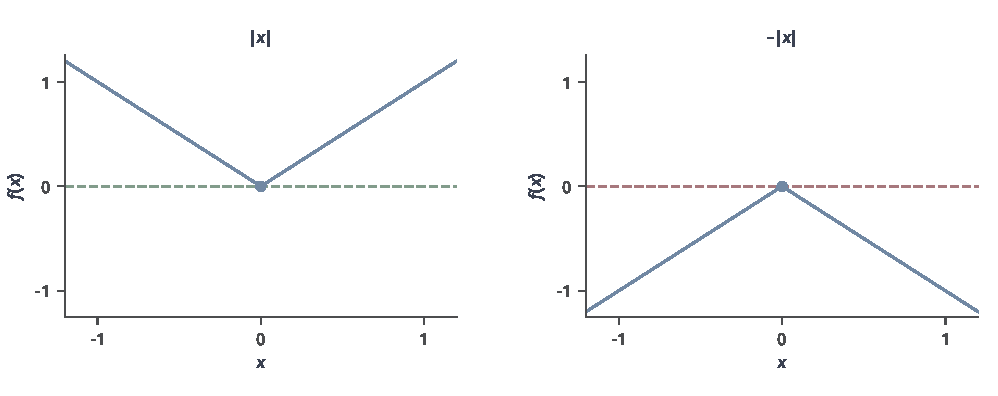
\includegraphics[width=169.0mm]{figures/00-shared/mathematical-preliminaries-upper/04-optimization/matplotlib/analysis-clarke-stationarity-boundary/figure.pdf}
  \caption{同一广义梯度区间$[-1,1]$的两种含义。蓝线分别为$|x|$与$-|x|$，虚线为原点候选斜率$g=0$的直线。左图候选直线在全局下界，右图原函数处处在直线下方。两图在原点都满足$0\in\partial^\circ f$，却分别是局部最小点和局部最大点。}
  \label{fig:analysis-clarke-stationarity-boundary}
\end{figure*}

\paragraph{含零必要性与最小性边界。}
局部极小点处，在移动基点差商中取固定基点$\bm y=\bm x$，所有足够小正$t$的分子非负，故$f^\circ(\bm x;\bm v)\geq0$对全部$\bm v$成立，由等价刻画得$0\in\partial^\circ f(\bm x)$，这是必要条件。反方向不成立：$-|x|$在原点是局部最大点而Clarke集合含零；若要求全域仿射下界，正半轴迫使$g\leq-1$、负半轴迫使$g\geq1$，斜率集合为空。局部Lipschitz凸函数的Clarke集合与凸次微分一致——只有恢复凸结构，才能引用12.6.2.1的全局判据。

\subsection{曲率条件不能互相替换}

用同一族二次函数隔离曲率条件的差别：
\[
 f_a(x_1,x_2)=\frac12(x_1+x_2)^2+\frac a2(x_1-x_2)^2.
\]
$a>0$时强凸；$a=0$时凸、满足PL但最小点成直线；$a<0$时弱凸而无下界。$f(x)=\cos x$二阶导数下界为$-1$，故为$1$弱凸却有无穷多个低点，在$x=0$梯度为零而目标差为$2$，没有正PL常数；前文的$f(x,y)=x^2+2\sin^2x$说明PL与弱凸可以共存。弱凸只限制可被二次距离补偿的负曲率，不保证全局最优、驻点唯一或收敛速度。

\begin{table*}[htbp]
 \centering\small
 \begin{tabularx}{\linewidth}{@{}lXX@{}}
 \toprule
 条件 & 直接控制什么 & 单凭该条件不能得到什么 \\
 \midrule
 凸性 & 全部线段上的弦上界；局部最小点也是全局最小点 & 最小点存在、最小点唯一或统一收敛速率 \\
 严格凸性 & 非平凡线段上的严格不等式；最小点至多一个 & 最小点存在，例$e^x$无最小点 \\
 强凸性 & 弦段与函数的二次间隔；目标差$\geq$距离平方界 & 梯度光滑性；例$|x|+\mu x^2/2$仍有尖点 \\
 弱凸性 & 最坏负曲率的可补偿下界 & 驻点全局最优或最小点唯一；$\cos x$有多个低点 \\
 PL条件 & 梯度平方控制目标差 & 凸性或参数唯一；可有多解与非凸景观 \\
 \bottomrule
 \end{tabularx}
 \caption{曲率条件的职责比较。各行针对不同性质，不能排成一条从“弱”到“强”的完整等级。}
 \label{tab:opt-curvature-conditions}
\end{table*}

\section{原问题的收敛速度与精度}

\subsection{原目标差与实际返回点}

凸问题、最小点存在且次梯度有界时，历史最佳点或加权平均点给$O(T^{-1/2})$目标差（预算未知的步长例多一对数因子）。精确邻近点法与凸邻近梯度法在各自精确子问题和合格步长下给最后一点$O(T^{-1})$，但一次调用是子问题而非一次廉价梯度读取。光滑化把原目标差拆成光滑优化误差与固定偏差$\nu\log m$；束方法以模型误差与到解距离控制中心。比较的是原目标误差与实际返回对象，阶数高不代表所有迭代点都更接近参数解。

\subsection{临界残差与全局目标差的边界}

光滑项失去凸性、非光滑项仍闭凸时，邻近梯度的历史最小平方梯度映射为$O(T^{-1})$（范数$O(T^{-1})$平方根即$O(T^{-1/2})$）；它控制复合临界性，不直接给最小值差，Clarke含零也只有必要性。目标差趋零、临界残差趋零、参数接近最小点是三件事，相互转换需要增长或误差界结构。

\subsection{预言器、子问题与精度预算}

复杂度先固定精度口径与计数单位：次梯度法的$O(\varepsilon^{-2})$是支撑读取数；精确邻近方法的$O(\varepsilon^{-1})$是子问题调用数；显式最大值的光滑化在统一距离界下普通／加速求解分别给$O(\varepsilon^{-2})$、$O(\varepsilon^{-1})$全梯度预算，还要按精度重选$\nu$与$L_\nu$；束方法既计实质步也计空步和随记忆增长的二次规划成本。这些阶数跨信息模型不能直接排序；不精确信息先按第14章明确误差来源与工作量。

\section{迭代过程与数值敏感度}

\subsection{原目标是否逐步改善}

\subsubsection{支撑更新不保证逐步下降}

12.2.3的三组反例——跨过尖点的大步、任意小步仍上升的负次梯度方向、尖点处不同支撑选择——共同否定逐轮下降推断。次梯度法的总体进展只能按历史最佳点或加权平均评价。

\subsubsection{由原目标比较保证的非增更新}

精确完整邻近点更新以旧点为候选，直接保证原目标非增并为位移付出正平方代价；精确邻近梯度在合格步长下由光滑上界与凸支撑使原复合目标非增，光滑项不凸也成立；束方法的实质步检验原$F$至少减少$\beta\Delta_k$，空步保持中心目标，查询点目标则可以上升。比较时要同时记录中心与查询点。

\subsubsection{只控制替代目标的光滑化更新}

普通梯度步在合格步长下使固定$F_\nu$下降，不能据此声称$F$逐步下降；加速更新甚至不承诺$F_\nu$逐步单调。应同时记录光滑替代值与原目标值，按两项误差界判断最终输出。

\subsection{目标进展能否推出参数收敛}

固定正步长、精确邻近更新且目标下有界时，累加下降式得平方位移可和、位移趋零，但这不证明路径总长度有限，也不单独给全序列收敛。在凸条件、固定步长与精确计算下，邻近比较使到任一原最小点的距离非增；目标差趋零配合有限维有界子列与闭目标，聚点落入解集，再由距离极限得全序列趋于其中一个解。多解时初值与规则可能选择不同解；次梯度法的最佳点或平均点界只评价返回序列。

\subsection{原解变化与计算扰动}

数据或正则参数改变时，首先比较两个原目标的最小点：适当闭$\mu$强凸$F$的线性扰动给$\|\bm w_{\bm b}-\bm w_{\bm c}\|_2\leq\|\bm b-\bm c\|_2/\mu$，不要求可微，但缺少原目标曲率时不能从邻近子问题唯一性推出此界。固定$r,\eta$时凸邻近映射非扩张只控制一次调用的中心误差；弱凸邻近输出可能放大误差；次梯度在尖点的不同选择可形成不同轨迹。原问题解集、一次调用与多步轨迹是三个对象，一般多步传播回用11.5的扩展状态框架。

\section{本章小结}

尖点处有四条求解路线：次梯度法读取一条全域支撑，邻近梯度法保留可求邻近的非光滑项，光滑化法用受控偏差取得单个光滑梯度，束方法积累下模型并核验原目标改善；邻近点法说明完整子问题的隐式更新。每步成本、是否逐步下降及最终返回对象都分别报告。

在原问题层面，存在性需要紧性或增长条件，唯一性需要原目标的额外结构；凸次微分含零给全局最优，Clarke含零一般只有必要性。目标差、平方驻点残差与参数收敛各有条件和评价对象。下一章中，指标函数的邻近映射将成为闭凸集投影，非光滑罚函数可调用本章方法，但原约束的可行性仍须独立检查。
